% Standalone XeLaTeX source. Uses standard commands and distributed packages.
% Source problem: public/notes/物工/問題/2017ap_exam.pdf, pages 9–10.
\documentclass[11pt,a4paper]{article}
\usepackage[margin=24mm]{geometry}
\usepackage{fontspec}
\usepackage{xeCJK}
\setCJKmainfont{HaranoAjiMincho-Regular.otf}
\usepackage{amsmath,amssymb}
\usepackage{tikz}
\usetikzlibrary{arrows.meta}
\setlength{\parindent}{1em}
\setlength{\parskip}{0.35em}
\title{物理工学専攻 院試解答集 ver2\\2017年 物理学II 第3問}
\author{政岡凜太郎}
\date{}
\begin{document}
\maketitle

\section*{[1.1] 二準位系の速度方程式}
上準位から下準位への遷移は自然放出と誘導放出、下準位から上準位への遷移は誘導吸収である。よって
\begin{align}
 \frac{dN_1}{dt}&=(A+BW(\omega_0))N_2-BW(\omega_0)N_1,\\
 \frac{dN_2}{dt}&=BW(\omega_0)N_1-(A+BW(\omega_0))N_2.
\end{align}
両式の和はゼロであり、全原子数密度$N_1+N_2$が保存する。

\section*{[1.2] 定常状態と占有数比}
定常状態では
\begin{equation}
 BW(\omega_0)(N_1-N_2)=AN_2.
\end{equation}
従って
\begin{equation}
 \boxed{W(\omega_0)=\frac{AN_2}{B(N_1-N_2)}},\qquad
 \frac{N_2}{N_1}=\frac{BW(\omega_0)}{A+BW(\omega_0)}<1.
\end{equation}
自然放出があるため、二準位系をこの放射場だけで駆動しても上準位の占有数は下準位を超えない。

\section*{[2.1] 空洞内の電磁波モード数}
一辺$d$の立方体に周期境界条件を置くと、許される波数は$\boldsymbol k=(2\pi/d)\boldsymbol n$（$\boldsymbol n\in\mathbb Z^3$）である。$|\boldsymbol k|\le\omega/c$を満たす格子点の数を、球の体積で近似する。各モードに横偏光が二つあるので
\begin{equation}
 N(\omega)=2\frac{d^3}{(2\pi)^3}\frac{4\pi}{3}\left(\frac{\omega}{c}\right)^3
 =\boxed{\frac{d^3\omega^3}{3\pi^2c^3}}.
\end{equation}

\section*{[2.2] モード密度とPlanck分布}
単位体積・単位角周波数あたりのモード数は
\begin{equation}
 D(\omega)=\frac{1}{d^3}\frac{dN}{d\omega}
 =\frac{\omega^2}{\pi^2c^3}.
\end{equation}
これに1モードあたりの平均エネルギーを掛ければ
\begin{equation}
 W_{\rm eq}(\omega)=D(\omega)\frac{\hbar\omega}{e^{\hbar\omega/(k_BT)}-1}
 =\boxed{\frac{\hbar\omega^3}{\pi^2c^3}\frac{1}{e^{\hbar\omega/(k_BT)}-1}}.
\end{equation}

\section*{[2.3] Einstein係数と共鳴周波数}
熱平衡では$N_2/N_1=e^{-\hbar\omega_0/(k_BT)}$である。[1.2]の定常式を用いると
\begin{equation}
 \frac{A}{B}=
 \left(\frac{N_1}{N_2}-1\right)W_{\rm eq}(\omega_0)
 =\left(e^{\hbar\omega_0/(k_BT)}-1\right)W_{\rm eq}(\omega_0).
\end{equation}
Planck分布を代入して温度依存性が消え、
\begin{equation}
 \boxed{\frac{A}{B}=\frac{\hbar\omega_0^3}{\pi^2c^3}}.
\end{equation}

\section*{[3.1] 三準位系の速度方程式}
図の矢印に沿って、ポンプ遷移$1\leftrightarrow3$、信号遷移$1\leftrightarrow2$、および$3\to2$の緩和を数えると
\begin{align}
 \frac{dN_1}{dt}&=-(P+L)N_1+(A+L)N_2+(A'+P)N_3,\\
 \frac{dN_2}{dt}&=LN_1-(A+L)N_2+CN_3,\\
 \frac{dN_3}{dt}&=PN_1-(A'+P+C)N_3.
\end{align}
三式の和はゼロで、$N_1+N_2+N_3$が保存する。遷移図は次の通りである。
\begin{figure}[htbp]
\centering
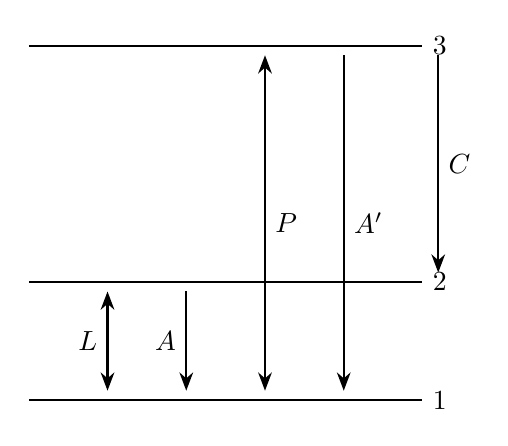
\begin{tikzpicture}[>=Stealth,thick]
 % Display heights encode energy ordering only; the spacings are schematic.
 \pgfmathsetmacro{\eOne}{0}
 \pgfmathsetmacro{\eTwo}{1.5}
 \pgfmathsetmacro{\eThree}{4.5}
 \draw (0,\eOne)--(5,\eOne) node[right] {$1$};
 \draw (0,\eTwo)--(5,\eTwo) node[right] {$2$};
 \draw (0,\eThree)--(5,\eThree) node[right] {$3$};
 \draw[<->] (1,\eOne+0.12)--(1,\eTwo-0.12) node[midway,left] {$L$};
 \draw[->] (2,\eTwo-0.12)--(2,\eOne+0.12) node[midway,left] {$A$};
 \draw[<->] (3,\eOne+0.12)--(3,\eThree-0.12) node[midway,right] {$P$};
 \draw[->] (4,\eThree-0.12)--(4,\eOne+0.12) node[midway,right] {$A'$};
 \draw[->] (5.2,\eThree-0.12)--(5.2,\eTwo+0.12) node[midway,right] {$C$};
\end{tikzpicture}
\caption{三準位系で考える遷移。上下位置はエネルギーの順序を示し、準位間隔は縮尺を表さない。}
\end{figure}

\section*{[3.2] 定常占有数比と反転条件}
定常状態で第3式から
\begin{equation}
 \frac{N_3}{N_1}=\frac{P}{A'+P+C}.
\end{equation}
これを第2式へ代入すると
\begin{equation}
 \boxed{\frac{N_2}{N_1}=
 \frac{(A'+P+C)L+CP}{(A'+P+C)(A+L)}}.
\end{equation}
この比が1を超える条件は、分子と分母の差を取って
\begin{equation}
 P(C-A)>A(A'+C)
\end{equation}
となる。従って反転が可能であるためには$C>A$が必要で、そのときのポンプ率の閾値は
\begin{equation}
 \boxed{P_c=\frac{A(A'+C)}{C-A}},\qquad P>P_c.
\end{equation}
$3\to2$緩和が$2\to1$の自然放出より速いと、準位2へ原子が効率よく蓄積し、十分なポンプで準位1より多くなる。$P=B_{13}W_p(\omega_p)$より反転条件は
\begin{equation}
 W_p(\omega_p)>\frac{A(A'+C)}{B_{13}(C-A)}.
\end{equation}

\section*{[3.3] 短波長ポンプで反転しにくい理由}
短波長化に対する困難は、問で与えられた三準位系の速度方程式から説明できる。準位$1\leftrightarrow2$の角周波数を$\omega_l$、ポンプ遷移$1\leftrightarrow3$を$\omega_p$とする。熱平衡Planck分布から得たEinstein関係をそれぞれの遷移に適用すると
\begin{equation}
 \frac{A}{B_{12}}=\frac{\hbar\omega_l^3}{\pi^2c^3},\qquad
 \frac{A'}{B_{13}}=\frac{\hbar\omega_p^3}{\pi^2c^3}.
\end{equation}
Einsteinの$B$係数を固定すれば、自発遷移率$A,A'$は対応する遷移周波数の三乗に比例して増加する。一方、反転に必要な条件は
\begin{equation}
 C>A,\qquad P>P_c=\frac{A(C+A')}{C-A}.
\end{equation}
実際、$C>A$の範囲では
\begin{equation}
 \frac{\partial P_c}{\partial A}=\frac{C(C+A')}{(C-A)^2}>0,\qquad
 \frac{\partial P_c}{\partial A'}=\frac{A}{C-A}>0.
\end{equation}
よって信号遷移の周波数$\omega_l$を上げると$A$が増し、閾値が上がるだけでなく、固定された緩和率$C$に対して最終的には$A\ge C$となり反転自体が不可能になる。ポンプ遷移の周波数$\omega_p$を上げても$A'$が増し、必要なポンプ率が増える。この説明はポンプ場のスペクトル形状を仮定しない。

なお、ポンプ光が別途熱平衡場だと仮定した場合に限り、Wien極限$\hbar\omega_p\gg k_BT$では
\begin{equation}
 W_{p,\mathrm{eq}}(\omega_p)\simeq\frac{\hbar\omega_p^3}{\pi^2c^3}
 e^{-\hbar\omega_p/(k_BT)}
\end{equation}
となり、高周波数での指数抑制も加わる。ただしこれは原問が置いていない追加条件である。
\end{document}
